 \documentclass{article}

\usepackage{geometry}
\usepackage{graphicx}
\usepackage{amsmath}

\title{Interfacing HD44780U LCD display and MCS-51 based microcontroller in EDISM simulator -- an EMISY laboratory}
\author{Maciej Marcinkiewicz (300171)}
\date{29th April 2021}

\newgeometry{lmargin=3.2cm, rmargin=3.2cm, bmargin=2.5cm}

\begin{document}

\maketitle

\section{Introduction}
\subsection{Brief description}
Laboratory's main purpose was to learn the basiscs of MCS-51 (Intel 8051) assembly
programming and to learn the way of proper dealing with 2x16 Hitachi HD44780U based displays.
The task was to use 8051 microcontroller to print some characters to the LCD.

\subsection{Schematic}
\begin{figure}[h!] %possible: b, t, h, p and override (!)
    \centering
        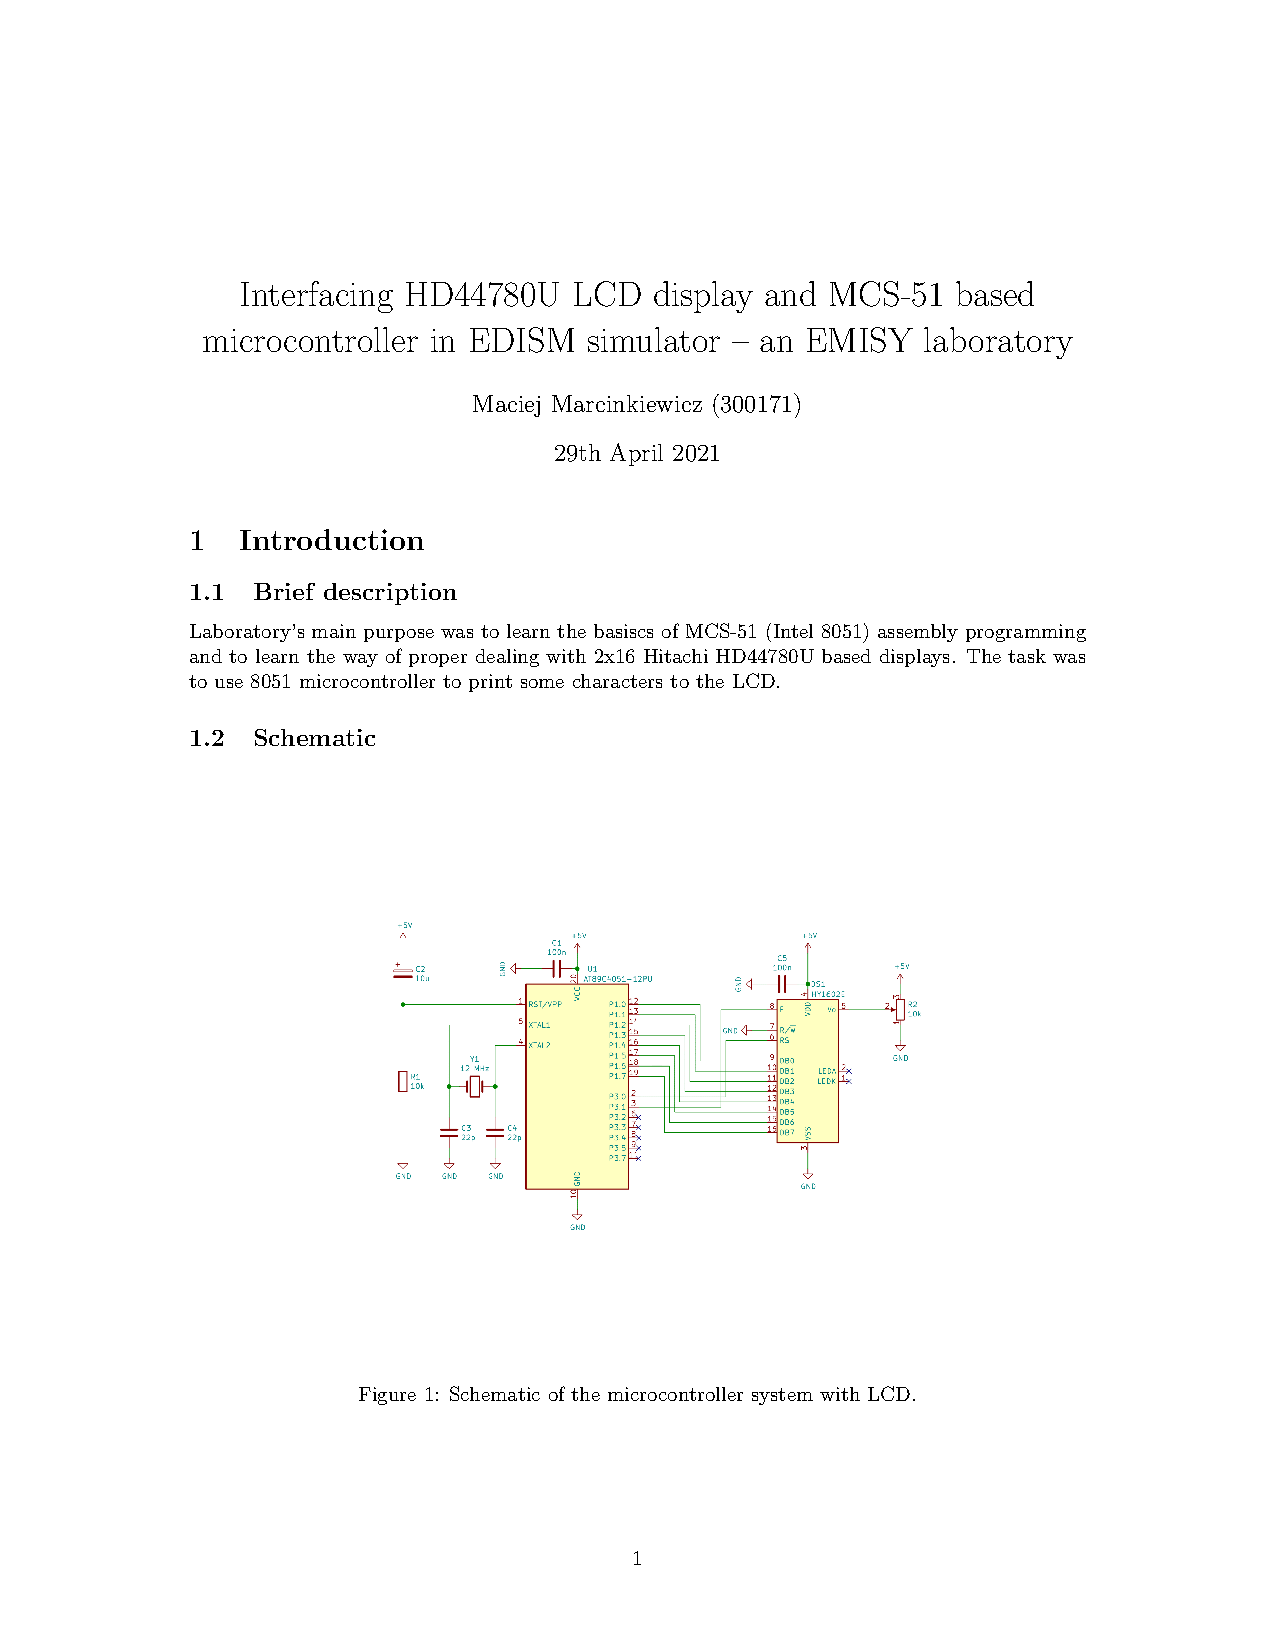
\includegraphics[width=0.9\linewidth]{schematics/lab1.png}
    \caption{Schematic of the microcontroller system with LCD.}
\end{figure}

\subsection{Hardware description}
Microcontroller (Atmel's AT89C4051) is connected to 5 V source and is equipped with 12 MHz clock and 
simple resetting circuit. LCD (HY1602E) is also connected to 5 V source. Its data bus is connected
to P1 GPIO port of the microcontroller unit. RS and E pins are connected to the P3.0 and P3.1,
respectively. LEDA and LEDK pins are not used. R/W pin is grounded, which corresponds to
permanent write (W) mode. Contrast pin V$_0$ is connected to the standard in this case 10 k$\Omega$ potentiometer.

\section{Task 1}
\subsection{Code description}

\end{document}